\documentclass{lab_sheet}
\usepackage[hidelinks]{hyperref}
\newcommand\ddfrac[2]{\frac{\displaystyle #1}{\displaystyle #2}}
\begin{document}
    \titlePage{Digital Modulation (ASK, FSK, BPSK and QAM)}{July 21, 2021}
    \pagenumbering{roman}
    \tableofcontents
    \clearpage
    \phantomsection
    \addcontentsline{toc}{section}{\bfseries{List of Figures}}
    \listoffigures
    \clearpage
    \phantomsection
    \addcontentsline{toc}{section}{\bfseries{Listings}}
    \lstlistoflistings
    \clearpage
    \pagenumbering{arabic}
    
\section{Objectives}
\begin{itemize}
    \item Perform and visualize amplitude shift keying, frequency shift keying, binary phase shift keying, quadrature amplitude modulation.
\end{itemize}


\section{Background Theory}
\subsection{Amplitude Shift Keying (ASK)}
ASK system is a digital modulation method where the bit '$1$' is represented by transmitting a sinusoidal carrier wave with fixed amplitude and frequency as $A_c$ and $f_c$ respectively for a bit duration of $T_b$ seconds, and the bit '$0$' is represented by turning off the carrier signal for $T_b$ seconds, which is why this method is also called \textit{On-Off Keying}. For a sinusoidal carrier wave $s_c(t)=A_c\cos(2\pi f_c t)$, the ASK signal is represented as,
\begin{equation}
    s(t)=\begin{cases}
        A_c\cos(2\pi f_c t)\quad &: \text{for bit } 1\\
        0 \quad &: \text{for bit } 0
    \end{cases}
    \label{eqn:ask}
\end{equation}
A generalized form of Equation~\ref{eqn:ask} for $x(t)=1 \text{ or } 0$ is,
\begin{equation}
    s(t)=x(t)A_c\cos(2\pi f_c t) \quad [0\leq t \leq T_b]
    \label{eqn:ask_general}
\end{equation}
We have, the signal power is given as, $P=\ddfrac{A_c^2}{2}$. For energy contained in a bit duration $E_b=PT_b$, Equation~\ref{eqn:ask_general} can be rewritten for bit '$1$' in the signal space diagram of ASK as,
\begin{equation}
    \begin{aligned}[b]
        s(t)&=\sqrt{2P} \cos(2\pi f_c t)\\
        s(t)&=\sqrt{PT_b} \sqrt{\frac{2}{T_b}} \cos(2\pi f_c t)\\
        s(t)&=\sqrt{E_b}\sqrt{\frac{2}{T_b}} \cos(2\pi f_c t)\\
        s(t)&=\sqrt{E_b} \Phi_1(t)
    \end{aligned}
    \label{eqn:ask_const}
\end{equation}
Equation~\ref{eqn:ask_const} shows that there is only one carrier function and the signal space diagram has two points on x-axis that are $\sqrt{E_b}$ apart.
\begin{figure}[H]
    \centering
    \includegraphics{../Figures/ask_const}
    \caption{Constellation diagram of ASK signal}
    \label{fig:ask_const}
\end{figure}

\begin{figure}[H]
    \centering
    \includegraphics{../Figures/ask_block}
    \caption{Block diagram for generation of ASK signal}
    \label{fig:ask_block}
\end{figure}

\subsection{Frequency Shift Keying (FSK)}
FSK system is a digital modulation method where two sinusoidal carrier waves of the same amplitude $A_c$  but different frequencies $f_{c1}$ and $f_{c2}$ are used to represent bits '$1$' and '$0$' respectively. For a sinusoidal carrier waves $s_{c1}(t)=A_c\cos(2\pi f_{c1} t)$ and $s_{c2}(t)=A_c\cos(2\pi f_{c2} t)$, the FSK signal is represented as,
\begin{equation}
    s(t)=\begin{cases}
        A_c\cos(2\pi f_{c1} t)\quad &: \text{for bit } 1\\
        A_c\cos(2\pi f_{c2} t) \quad &: \text{for bit } 0
    \end{cases}
    \label{eqn:fsk}
\end{equation}
A generalized form of Equation~\ref{eqn:fsk} is, 
\begin{equation}
    s_i(t)=\begin{cases}
        \sqrt{\ddfrac{2E_b}{T_b}}\cos(2\pi f_{ci} t) \quad &[0\leq t \leq T_b]\\
        0 \quad &\text{elsewhere}
    \end{cases}
    \label{eqn:fsk_general}
\end{equation} 
For FSK system the signal space diagram has two message points and is two dimensional.
\begin{figure}[H]
    \centering
    \includegraphics{../Figures/fsk_const}
    \caption{Constellation diagram of FSK signal}
    \label{fig:fsk_const}
\end{figure}

\begin{figure}[H]
    \centering
    \includegraphics[scale=0.8]{../Figures/fsk_block}
    \caption{Block diagram for generation of FSK signal}
    \label{fig:fsk_block}
\end{figure}

\subsection{Binary Phase Shift Keying (BPSK)}
BPSK system is a digital modulation method where both the bits '$1$' and '$0$' are represented by transmitting a sinusoidal carrier wave with fixed amplitude and frequency as $A_c$ and $f_c$, except the carrier phase of each bit differs bt $\pi$. For a sinusoidal carrier wave $s_c(t)=A_c\cos(2\pi f_c t)$, the BPSK signal is represented as,
\begin{equation}
    s(t)=\begin{cases}
        A_c\cos(2\pi f_c t)\quad &: \text{for bit } 1\\
        A_c\cos(2\pi f_c t+\pi)\quad &: \text{for bit } 0\\
    \end{cases}
    \label{eqn:bpsk}
\end{equation}
A generalized form of Equation~\ref{eqn:bpsk} for $$b(t)=\begin{cases}
    +1 \quad & \text{when binary '1' is to be transmitted}\\
    -1 \quad & \text{when binary '0' is to be transmitted}\\
\end{cases}$$ \\is given as,
\begin{equation}
    s(t)=b(t)A_c\cos(2\pi f_c t) \quad [0\leq t \leq T_b]
    \label{eqn:bpsk_general}
\end{equation}
We have, the signal power is given as, $P=\ddfrac{A_c^2}{2}$. For energy contained in a bit duration $E_b=PT_b$, Equation~\ref{eqn:bpsk_general} can be rewritten as,
\begin{equation}
    \begin{aligned}[b]
        s(t)&=\pm\sqrt{2P} \cos(2\pi f_c t)\\
        s(t)&=\pm\sqrt{PT_b} \sqrt{\frac{2}{T_b}} \cos(2\pi f_c t)\\
        s(t)&=\pm\sqrt{E_b}\sqrt{\frac{2}{T_b}} \cos(2\pi f_c t)\\
        s(t)&=\left\{[\sqrt{E_b} \Phi_1(t)],[-\sqrt{E_b} \Phi_1(t)]\right\}
    \end{aligned}
    \label{eqn:bpsk_const}
\end{equation}
\begin{figure}[H]
    \centering
    \includegraphics{../Figures/psk_const}
    \caption{Constellation diagram of BPSK signal}
    \label{fig:bpsk_const}
\end{figure}

\begin{figure}[H]
    \centering
    \includegraphics{../Figures/psk_block}
    \caption{Block diagram for generation of BPSK signal}
    \label{fig:bpsk_block}
\end{figure}
\subsection{Quadrature Amplitude Modulation (QAM)}
QAM system is a digital modulation method where variation in phase (similar to M-ary PSK) as well as amplitude is used to carry information of the message signal.
\begin{equation}
    s(t)=\begin{cases}
        \sqrt{\ddfrac{2E_b}{T_b}}a_i \cos(2\pi f_c t)+\sqrt{\ddfrac{2E_b}{T_b}}b_i \sin(2\pi f_c t)\quad &[0\leq t \leq T_b]\\
        \quad 0 &\text{elsewhere}
    \end{cases}
    \label{eqn:qam_general}
\end{equation}
where, $E_b$ is the energy of the lowest amplitude signal, $a_i$ and $b_i$ are pair of independent integers that are chosen based on the position of message points. The coordinates of the $i^{th}$ message point are $a_i\sqrt{E_b}$ and $b_i\sqrt{E_b}$ where $(a_i,b_i)$ is an element of the $L\times L$ matrix, where $L=\sqrt{M}$, and $M$ is the number of symbols used.
\begin{equation}
   (a_i,b_i)= \begin{bmatrix} 
        (-L+1,L-1) & (-L+3, L-1) & \dots & (L-1,L-1) \\
        (-L+1,L-3) & (-L+3, L-3) & \dots & (L-1,L-3) \\
        \vdots & \vdots & \vdots & \vdots \\
        (-L+1,-L+1) & (-L+3, -L+1) & \dots & (L-1,-L+1)
      \end{bmatrix} 
\end{equation}
\begin{figure}[H]
    \centering
    \includegraphics[width=\linewidth]{../Figures/qam_const}
    \caption{Constellation diagram of M-ary QAM signal}
    \label{fig:qam_const}
\end{figure}

\begin{figure}[H]
    \centering
    \includegraphics{../Figures/qam_block}
    \caption{Block diagram for generation of M-ary QAM signal}
    \label{fig:qam_block}
\end{figure}
\section{Exercises}
\matlabcode{bitgenerator}{Matlab script for generating bit sequence}

\mysub{Amplitude Shift Keying (ASK)}
\problem{Perform and visualize ASK modulation.}
\matlabcode{ask}{Matlab script for amplitude shift keying digital modulation}
\begin{figure}[H]
    \centering
    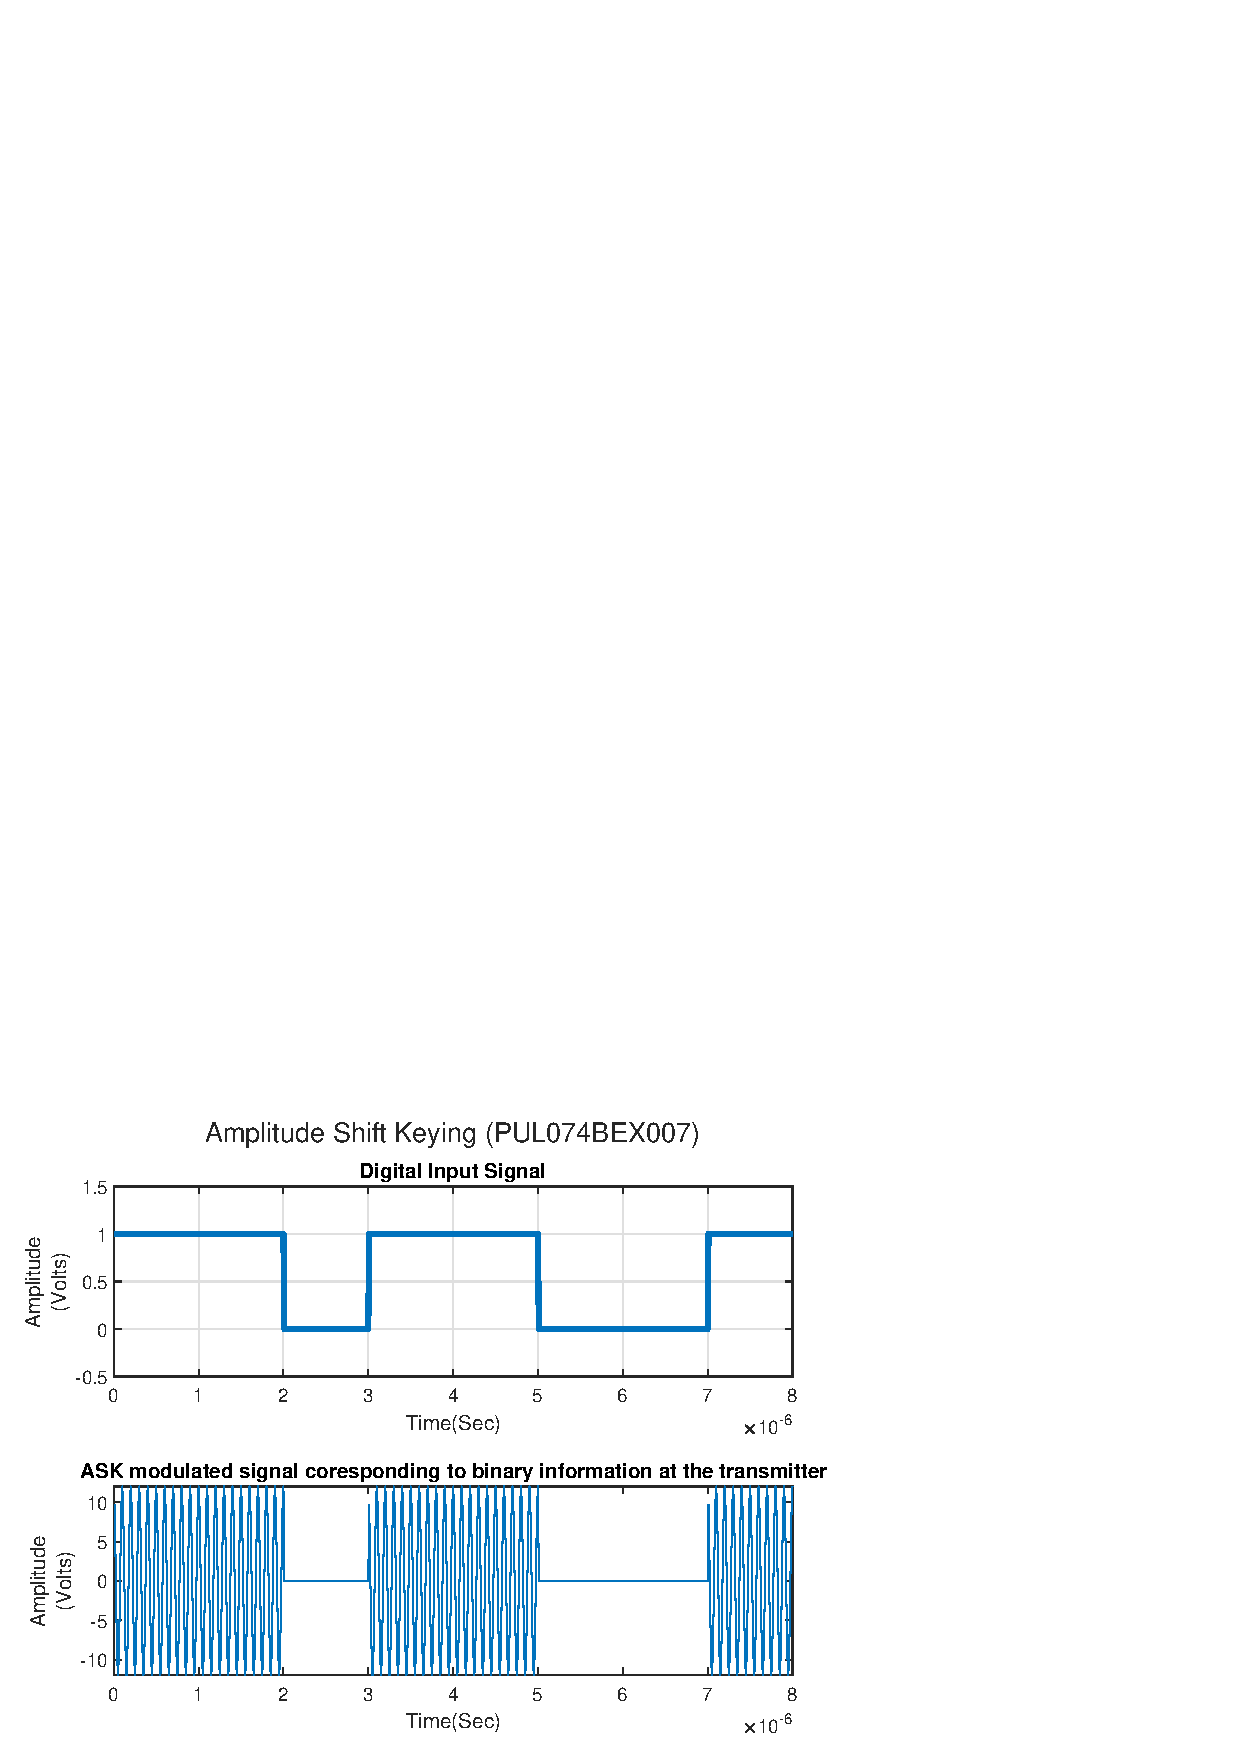
\includegraphics{../Figures/ask-obs}
    \caption{Observation for ASK digital modulation}
    \label{fig:ask-obs}
\end{figure}

\mysub{Frequency Shift Keying (FSK)}
\problem{Perform and visualize FSK modulation.}
\matlabcode{fsk}{Matlab script for frequency shift keying digital modulation}
\begin{figure}[H]
    \centering
    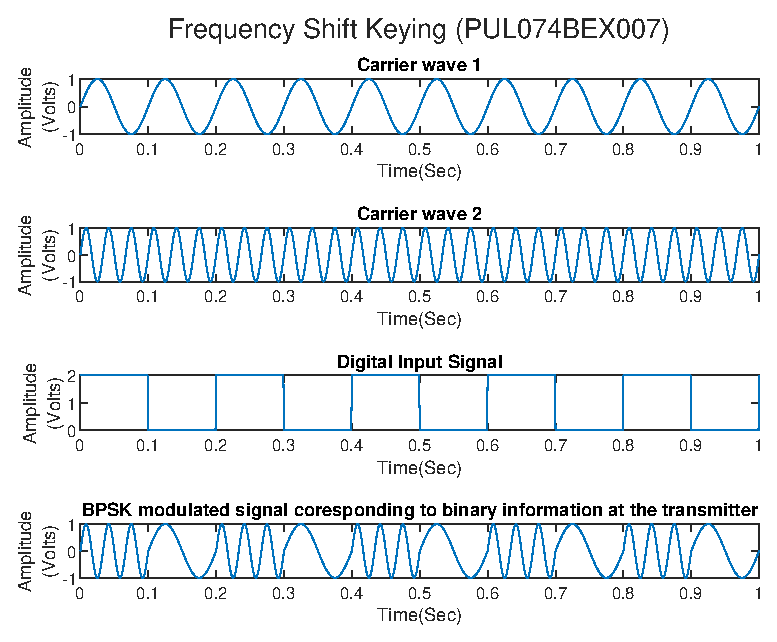
\includegraphics{../Figures/fsk-obs}
    \caption{Observation for FSK digital modulation}
    \label{fig:fsk-obs}
\end{figure}

\mysub{Binary Phase Shift Keying (BPSK)}
\problem{Perform and visualize BPSK modulation.}
\matlabcode{psk}{Matlab script for binary phase shift keying digital modulation}
\begin{figure}[H]
    \centering
    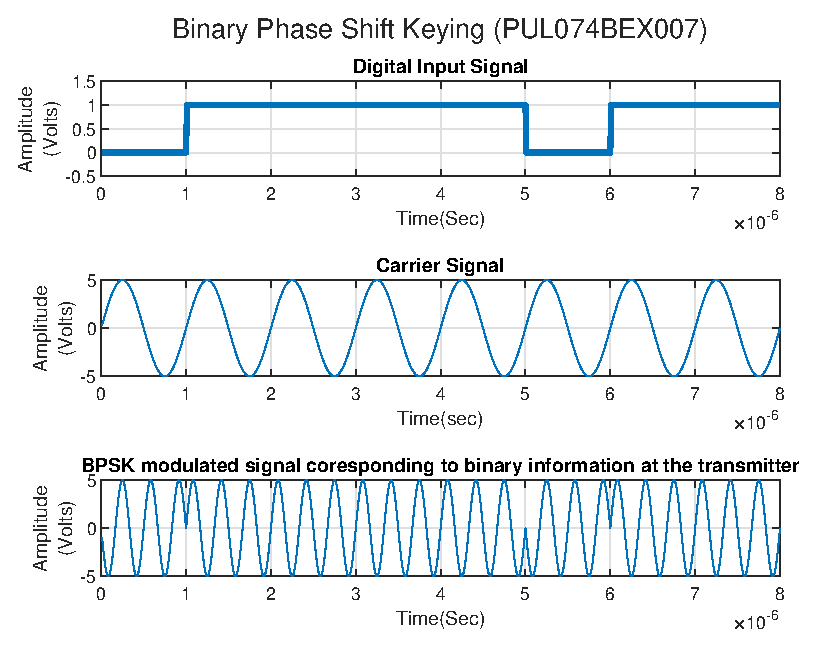
\includegraphics{../Figures/psk-obs}
    \caption{Observation for BPSK digital modulation}
    \label{fig:bpsk-obs}
\end{figure}

\mysub{Quadrature Amplitude Modulation (QAM)}
\problem{Perform and visualize QAM.}
\matlabcode{qam}{Matlab script for quadrature amplitude modulation}
\begin{figure}[H]
    \centering
    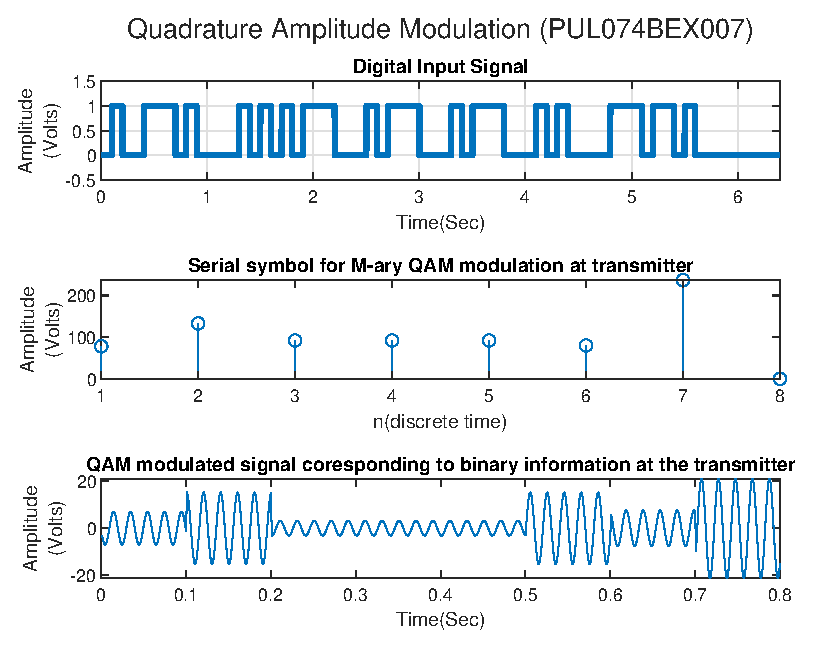
\includegraphics{../Figures/qam-obs}
    \caption{Observation for QAM (256-ary)}
    \label{fig:qam-obs}
\end{figure}

\section{Discussion and Conclusion}
This lab experiment dealt with the implementation and visualization of different digital modulation schemes like amplitude shift keying, frequency shift keying, binary phase shift keying, and quadrature amplitude modulation. \\
A single bit generator script was used for ASK and BPSK modulation, whereas a different method to generate the input digital signal was implemented for FSK modulation. This was done solely for experimental purposes. Likewise, for the QAM scheme, a digital signal represented by 64 bits was generated for 256-ary QAM scheme using a technique similar to the script for ASK and BPSK. Moreover, the serial symbol conversion was performed using \verb|reshape| command. The reshaped information provided the serial symbol which was converted from the rows of the reshaped matrix into decimal system. \verb|qammod| command was used to perform QAM scheme which gave back the real and imaginary parts, using which the QAM signal was represented and plotted as shown in the observation above.\\
Hence the objectives of the lab experiment were fulfilled with the implementation and visualization of ASK, FSK, BPSK and QAM.
\end{document}